\documentclass[conference]{IEEEtran}

\usepackage{epsfig}
\usepackage{fancyvrb}
\usepackage{url}

\DefineVerbatimEnvironment%
  {code}{Verbatim}{numbers=left,numbersep=3pt,frame=lines,%
                   xleftmargin=7pt,fontsize=\footnotesize}




\begin{document}


\title{A Component-Based Sensor Network for \\ Environmental Monitoring}

\author{\authorblockN{A. Puder, T. Johnson, K. Sales, M. de Sales}
\authorblockA{San Francisco State University \\
Computer Science Department \\
1600 Holloway Avenue \\
San Francisco, CA 94132 \\
EMail: \{arno$\mid$tlj$\mid$klebers$\mid$msales\}@sfsu.edu}
\and
\authorblockN{D. Robinson}
\authorblockA{San Francisco State University \\
Romberg Tiburon Center \\
3150 Paradise Drive \\
Tiburon, CA 94920 \\
EMail: dhr@sfsu.edu}}


\maketitle
\begin{abstract}
  In this paper we describe a sensor network for environmental
  monitoring based on highly specialized, off-the-shelf sensing
  devices.  Environmental monitoring depends on the reliable
  collection of measurements from remotely deployed sensors and the
  rapid transfer of those measurements to data centers. Typically,
  sensors are deployed in out-of-the-way locations, where physical
  access is limited and connections for telemetry are poor or
  nonexistent. Maintaining the data stream from these sensors places
  demands on human resources, requiring site visits to service the
  sensors and to download data stored on internal memory.  The work
  described in this paper is a collaborative effort between the
  Computer Science Department at San Francisco State University and
  the Romberg Tiburon Center. The result of this collaboration is an
  environmental sensor network deployed in the San Francisco Bay. It
  provides means to program and interrogate sensors at the remote
  field locations and to transmit collected measurements to a remote
  database.
\end{abstract}


\section{Introduction}

A wireless sensor network consists of spatially distributed autonomous
devices using sensors to cooperatively monitor physical or
environmental conditions at different locations \cite{roemer:2004}.
Much research effort is focused on building wireless ad-hoc networks
where each sensor node participates in a multi-hop routing algorithm.
One the earliest examples of a wireless sensor network is the
SmartDust project \cite{smartdust:2001} where one objective was to
create autonomous sensing and communication in a cubic
millimeter-sized device.  While most wireless sensor networks focus on
small sensing devices such as the SmartDust mote, there exist a wide
variety of off-the-shelf commercially available sensors that are used
by environmental researchers. In contrast to the small sensing
devices, sensors for environmental monitoring are typically on the
order of one to two feet in length weighing several pounds. Our
focus is on building an end-to-end infrastructure for environmental
monitoring using specialized sensing devices.

Environmental monitoring depends on the reliable collection of
measurements from remotely deployed sensors and the rapid transfer of
those measurements to data centers. Typically, sensors are deployed in
out-of-the-way locations, where physical access is limited and
connections for telemetry are poor or nonexistent. Maintaining the
data stream from these sensors places demands on human resources,
requiring site visits to service the sensors and to download data
stored on internal memory.  Consequently, there is a lag of days to
months between the time the sensors perform the measurements and the
time the measurements become available. Advances in battery life and
anti-fouling technology have extended service cycles for field
sensors, with the unwanted result of further delaying access to
monitoring data.  In addition, the dependence on field site visits to
alter of sensor characteristics, such as sampling rate, prevents
adjustment in monitoring strategy in response to rapidly developing
events (e.g. oil spills, harmful algal blooms).

The work described in this paper is a collaborative effort between the
Computer Science Department at San Francisco State University and the
Romberg Tiburon Center (RTC), a research institute focusing on the
understanding of complex marine and estuarine environments. The result
of this collaboration is NetBEAMS (Networked Bay Environmental
Assessment Monitoring System), an environmental sensor network
deployed in the San Francisco Bay. NetBEAMS provides means to program
and interrogate sensors at the remote field locations and to transmit
collected measurements to a database, where the data is rapidly
processed, archived, and made available to potential users in near
real-time. In the following we give an overview of the NetBEAMS
architecture and implementation.  Section \ref{SEC_BACKGROUND}
describes a typical environmental sensor used by the RTC. Section
\ref{SEC_DSP} describes our Data Sensor Platform (DSP) that allows us
to efficiently build up an end-to-end environmental sensor network.
Section \ref{SEC_NETBEAMS} describes NetBEAMS; a practical application
of the DSP. In Section \ref{SEC_CONCLUSION} we provide a conclusion
and outlook.


\section{Background}
\label{SEC_BACKGROUND}

Environmental researchers typically use standard, off-the-shelf
sensing devices for their purposes. These sensing devices are at the
opposite spectrum of miniature sensors such as SmartDust. One such
device is the YSI 6600EDS V2 Sonde \cite{Sonde01}. It is a water
quality monitoring device that gathers water quality data, and
operates in fresh, sea, or polluted water. Some of the measurements
that the YSI is capable of are conductivity, temperature, chloride,
ammonium, nitrate, turbidity, and chlorophyll.  It is under 55 cm in
length, 8.9 cm in diameter, and weighs approximately 3.18 kg. It
operates at temperatures between -5 to +50 deg C and at depths up to
200 meters.  It uses 8 C-size Alkaline Batteries or External 12 VDC.
Battery life can last up to 75 days depending on sensor configuration.
The Sonde's bulkhead contains multiple pin connectors to support
sensor probes for measuring parameters as shown in Table
\ref{TAB_SONDE_MEASUREMENTS}.

\begin{table}[h]
\caption{\label{TAB_SONDE_MEASUREMENTS} YSI Sonde measurements.}
\centering
\begin{tabular}{|l||l|}
\hline
\multicolumn{1}{|c||}{\textbf{Name}} &
\multicolumn{1}{c|}{\textbf{Description}} \\ \hline \hline
\texttt{Date}    & Year/Month/Day. \\ \hline
\texttt{Time}    & Hour:Minute:Second. \\ \hline
\texttt{Temp}    & Temperature in degrees Celcius. \\ \hline
\texttt{SpCond}  & Specific Description in microSiemens
                   per centimeter. \\ \hline
\texttt{Cond}    & Conductivity in microSiemens per centimeter. \\ \hline
\texttt{Resist}  & Resistivity in Ohms $*$ centimeter. \\ \hline
\texttt{Sal}     & Salinity in parts per thousand. \\ \hline
\texttt{Press}   & Pressure in pounds per square inch relative. \\ \hline
\texttt{Depth}   & Water column in meters. \\ \hline
\texttt{pH}      & pH in standard units. \\ \hline
\texttt{phmV}    & millivolts associated with the pH reading. \\ \hline
\texttt{ODOSat}  & Dissolved oxygen in \% air saturation. \\ \hline
\texttt{ODOConc} & Dissolved oxygen in mg/L. \\ \hline
\texttt{Turbid}  & Turbidity in nephelometric turbidity units. \\ \hline
\texttt{Battery} & Total Volts remaining in batteries.  \\ \hline
\end{tabular}
\end{table}


Each probe may have multiple sensors.  A computer can interface with
the Sonde via RS-232C or SDI-12. The Sonde can be configured to
collect data samples in discrete or unnattended mode.  Discrete mode
is normally performed while a technician manages the Sonde during the
sampling process. In this mode the Sonde is usually connected via 650
MDS Display/Logger or a serial cable connected to a PC.  The sampling
frequency is usually set to a high frequency in this mode.  Unattended
mode is performed usually when the Sonde is deployed offshore or in a
remote body of water.  The sampling frequency is usually set for a
longer period of time (i.e. 5 - 15 min). The Sonde is configured via a
set of menus that can be accessed through a terminal session over
RS232. Through these menus, the Sonde can be configured to start
logging data to an internal file.  To view the data as it's being
captured, the option to show live data is chosen and the data can then
seen via a serial terminal session at each interval.

We provide these details to show that sensing devices such as the YSI
are highly specialized devices with a unit price of several thousand
dollars. These sensors are usually sparsely deployed in remote
locations that not only make their maintenance difficult, but also
access to their measurements.  Typically, the sensors are autonomous
in the sense that they can run for a certain time on battery power and
store the measurement data in internal memory. Only when the sensors
are serviced, the measurement data, which was collected since the last
servicing, is uploaded to a portable storage device. From there, the
data can be uploaded to server. This manual procedure to retrieve
sensor data is not only error prone, but also results are in a serious
time lag between the time the sensor performs the measurement and when
it becomes available for further processing. For many applications,
however, it would be beneficial to have near-realtime access to the
sensor measurement. We identify the following requirements that an
end-to-end infrastructure supporting devices such as the YSI should
offer:

\begin{itemize}
\item Allow near-realtime access to sensor measurements.
\item Allow remote servicing that include changing of configuration
  parameters as well as software upgrades.
\item Support cost-effective long distance communication link.
\item Can be deployed in remote locations in unprotected outdoor
  conditions.
\end{itemize}

In the next section we describe a software architecture that provides
a foundation to fulfill these requirements.


\section{Data Sensor Platform}
\label{SEC_DSP}

Sensor networks, especially of environmental sensors, are normally
deployed over a geographically wide area where the communication
infrastructure is not always reliable or, at least, not countinuously
available. As the sensor network grows in size and complexity
scalability, reliabilty and maintainability become critical issues.
Additional components might be added to the network, sensor
configuration might be altered, or new versions of components might be
deployed. The sensor network must be able to support such adjustments
without significant overhead for maintainers.  From system
development and integration point of view, interfaces among components
and between components and the network should be simple. Complex
interaction can be constructed on top of these simple interfaces.  In
the following we discuss how our proposed architechure addresses those
issues.

\subsection{Architecture}

Our architecture is based on a micro-kernel approach. The core
functionality is limited to a minimum and all extra services are built
as plug-and-play modules on top of the micro-kernel. With the help of
this approach we can keep the basic infrastructure compact while
allowing customization via special-purpose modules. In our terminology
we call the basic foundation the \emph{Data Sensor Platform}
(DSP). The scope of the DSP is one address space of an execution
platform. A sensor network is built from several DSPs that are linked
with each other.

Figure \ref{FIG_DSP} depicts the basic architecture of the DSP. We
refer to the plug-and-play modules as DSP Components. DSP Components
are self-contained modules that can be added and removed to a DSP
installation at runtime. The basic communication paradigm within a DSP
is a message. DSP Components can exchange messages of different types.
Actually, all interactions between DSP Components are implemented
through messages yielding simple but powerful communication
instructure.  We distinguish between \emph{Data Producers} (DP) and
\emph{Data Consumers} (DC) within the scope of a DSP. DP and DC can be
seen as roles that a DSP Component may have. It is possible for a DSP
Component to act in the role of DC and DP at the same time. Messages
in DSPs are routed based on rules. Rules can be configured statically
or dynamically. Rules for routing messages can be based on different
information: producers or consumers of the message, the message
itself, or specific configuration parameters provided externally.

\begin{figure}
\centering
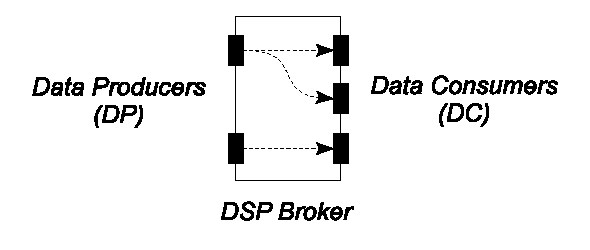
\epsfig{file=dsp, width=7cm}
\caption{\label{FIG_DSP} Data Sensor Platform (DSP).}
\end{figure}

The DSP is responsible for routing messages between DPs and DCs. It is
important to note that this routing only happens within a
DSP. Following the paradigm of a micro-kernel approach, the DSP has no
notion of remote communication or sensor-specific details. All this
knowledge is embodied in special purpose DSP Components.

\subsection{DSP Components}

A DSP Component encapsulates a particular functionality. We
distinguish between those components that produce data (DP) and those
that consume data (DC). An example for a DSP Component acting in the
role of a DP is a module that interfaces with a physical sensor. Such
a module reads data from the sensor and converts the data into a
message that is forwarded to the DSP. Because this module generates
data with respect to the DSP, it is a data producer. An example for a
data consumer is a converter module that converts the internal,
DSP-specific data format to a format suitable for consumption by
external applications. One such common format used in the domain of
environmental monitoring is OpenDAP \cite{opendap01}.  Since the
converter module accepts messages from the DSP, it acts in the role of
a data consumer. Finally, a DSP Component implementing persistency is
an example of a module that acts in the roles of both data producer
and consumer. It accepts messages from the DSP and stores them in a
database. At a later time, it may act as a data producer by resending
previously stored messages.

All DSP Components need to implement the following Java interface:

\begin{code}
interface DSPComponent
{
   public String getComponentType();
   public void initComponent(...);
   public void startComponent();
   public void stopComponent();
   public void deliver(DSPMessage msg);
   // ...
}
\end{code}

By implementing the above Java interface, the resuling code
effectively becomes a DSP Component that can be deployed on a DSP at
runtime. A component is identified by its type (line 3). Only one
component of a certain type per DSP is permissible. A type identifier
must be unique across all DSP Components in a DSP.  Upon deploying a
component, an initialization function is called (line 4). Once a
component is initialized, it may be started (line 5) and stopped (line
6) multiple time. Whenever the DSP wishes to pass a message (that was
generated by some DP), it invokes the \texttt{deliver()} method (line
7). The message structure will be explained in the following section.
One important feature of the DSP is the ability to redeploy (maybe
with a new version) at runtime. This allows DSPs to be updated
remotely. This process is managed through messages sent to a special
DSP Component that is able to manage its local DSP.

\subsection{Message Structure}

Message passing is the main paradigm for exchanging information within
a DSP. After producing data, a DP wraps that data in the body
of a message, so that DC components can receive the message and
consume the data contained in the message's body. When it comes to passing
messages to a remote DSP instance, messages are serialized in XML
\cite{xml2000} and automatically deserialized for DC located in the
remote DSP. In order to serialize and deserialize DSP messages, the
DSP infrastructure uses the XML Schema standard \cite{xml-schema2004}
to generate and validate the DSP message. Figure \ref{FIG_DSP_MESSAGE}
defines the structure of a general DSP message.

\begin{figure}[!htb]
 \centering
 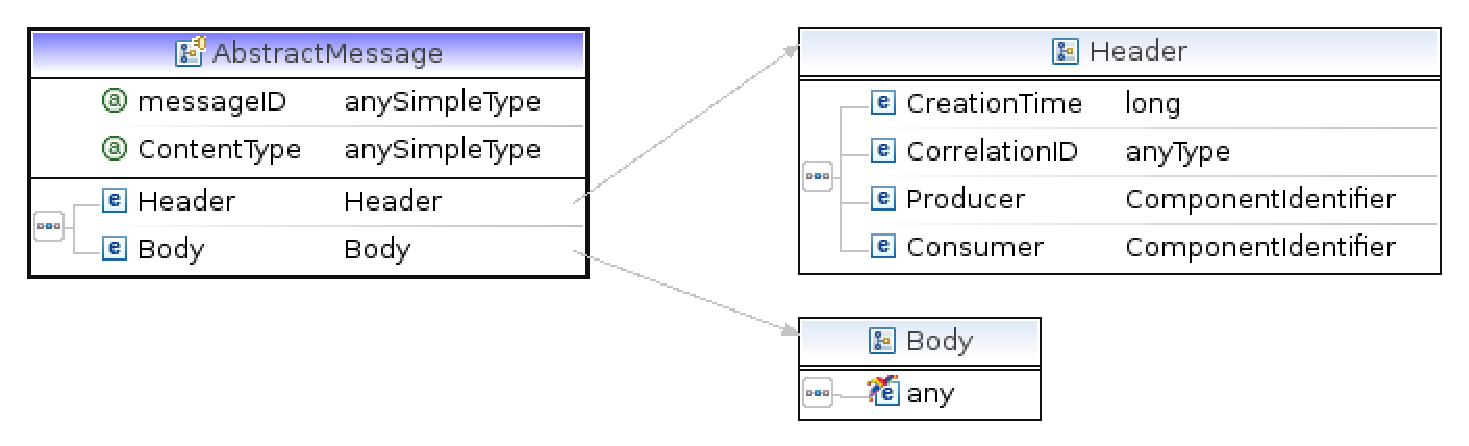
\epsfig{file=dsp-message, width=9cm, height=4cm}
 \caption{\label{FIG_DSP_MESSAGE} Structure of a DSP message.}
\end{figure}

The basic message structure is defined by an \texttt{AbstractMessage}
type, whose structure serves as a base schema for all different types
of messages. Any message will contain two basic attributes:
\texttt{messageID} and \texttt{ContentType}.  The former uniquely
identifies a message and the latter the data in the body of the
message. Complementary identification information such as the message
producer and consumer are located in the header of the message, which
are defined by the schema type \texttt{ComponenIdentifier}. A
\texttt{ComponentIdentifier} carries out information about the
component name and its physical host address.  Finally, the body of
the message represents the payload and may contain any data type
defined by the component developer.

Although XML schema is the de-facto standard to bind and validate XML
data to its type, the architectural infrastructure of DSP uses an XML
data binding technology \cite{xml-dbind} called JAXB \cite{xml-jaxb}.
It is used to generate a type safe API for handling in-memory object
graphs from the XML instances of DSP Messages and the content of its
data payload. Moreover, taking advantage of the data type polymorphism
of XML schema data types -- a concept borrowed from object oriented
principles -- we defined different categories of messages in order to
reflect the nature of the message content. Among those categories are
query and update messages for configuring various properties supported
by DSP Components and measurement messages that actually contain
sensor readings.

The payload of a message is itself described via an XML schema in
order to integrate it seemingly with the general message structure. A
developer of a DSP Component can define a schema that represents the
type of payload processed by that component. An example illustrating a
DSP message is given when we discuss the YSI Sonde Component.

\subsection{DSP Broker}

In order to keep the API symmetrical, the DSP is itself implemented as
a DSP Component, the so-called DSP Broker. While technically the DSP
Broker has the same API as any component, it serves a special role and
cannot be removed. When a DP sends a message, it actually
invokes the \texttt{deliver()} method of the DSP Broker. The broker is
responsible for routing the message to one or several DCs. It
distinguishes between local and remote destinations:

\begin{itemize}
\item Local delivery of messages: it uses local object reference to
  deliver the DSP message.
\item Remote delivery of messages: it uses a DSP Component marked as a
  default gateway to handle remote message delivery.
\end{itemize}

The selection of the DCs for a given message to where the broker will
deliver messages to is determined by a matcher.  The matcher is
responsible to find the possible set of DCs for a given DSP message,
and it relies on matching rules defined statically or at runtim. In
this way, a set of matching rules is defined in XML and stored at the
DSP run-time directory, where each matching rule is uniquely
identified by a rule ID and determines the following (see Figure
\ref{FIG_MATCHER_RULE}):

\begin{figure}[!htb]
 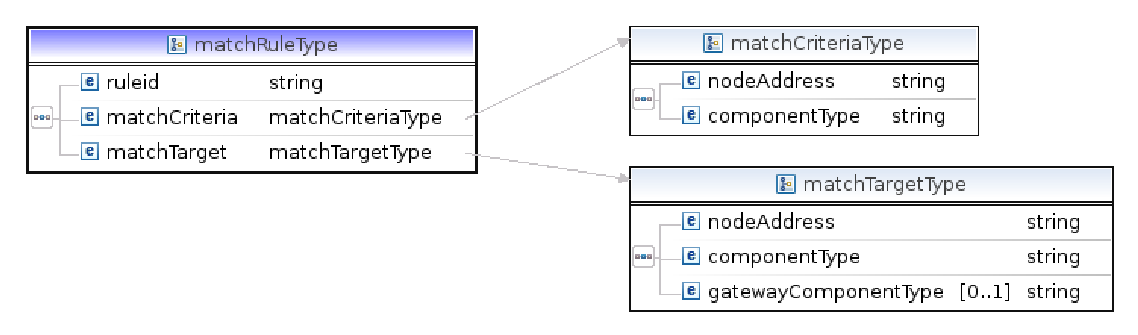
\epsfig{file=dsp-match-rule, width=9cm, height=4cm}
 \caption{\label{FIG_MATCHER_RULE} Definition of Matcher Rule.}
\end{figure}

\begin{itemize}
\item The \emph{match criteria} defines the name of the component type
  of the producer and its physical location (IP address);
\item The \emph{match target} defines the name of the component type
  of the consumer, and optionally defines a gateway component.
\end{itemize}

When analyzing the matching rules, the matcher only selects the rules
that satisfy the matching criteria and forwards them back to the
broker. Once the broker has the matching rules, it determines whether
the delivery is done directly to a component defined on the match
target, or if the message is delivered to the optional gateway. We
have defined special gateway DSP components that is used to transport
the DSP Messages, serialized in XML, to any remote DSP instance.


\section{NetBEAMS}
\label{SEC_NETBEAMS}

\begin{figure*} 
\centering
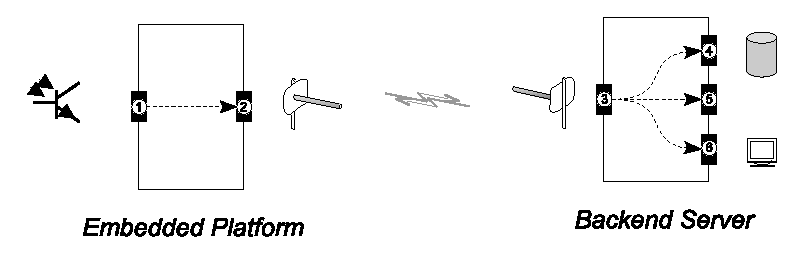
\epsfig{file=netbeams, width=14cm}
\caption{\label{FIG_NETBEAMS} NetBEAMS architecture.}
\end{figure*}

In the following we present a practical application of the DSP
presented in the previous section. We describe a deployment of the DSP
using sensor owned and operated by the RTC. Our environmental sensor
network is dubbed NetBEAMS (Networked Bay Environmental Assessment
Monitoring System) and allows access to sensor equipment deployed
throughout the San Francisco Bay Area.  Our goal is to address the
problem of data collection from remote sensors by using the DSP to
automatically interrogate sensors at the remote field locations and
transmit the collected measurements over long distances to a backend
server where the data is made available to potential users in near
real-time. This end-to-end system will be a ready-to-use turnkey
solution that is adaptable to a wide variety of sensor types and
requires no programming expertise to operate. Configuration of the
system will be possible when the sensor is deployed in the field via a
web-based interface, eliminating the need for extra site visits by
technicians between service cycles to change systems functionalities
(e.g. sampling rate). We present the NetBEAMS infrastructure by
discussing its hardware and software components.


\subsection{Hardware}

Figure \ref{FIG_NETBEAMS} provides an end-to-end overview of the
NetBEAMS architecture. NetBEAMS is built using multiple installations
of the DSP and by providing special purpose components for the various
tasks. One DSP installation is collocated with each sensor and an
additional DSP is running on the backend server. Because of the remote
locations where each individual sensor is deployed in the field and
the sparse nature of the network, the resulting topology is a tree
structure of depth 1.

NetBEAMS supports an environmental sensor such as the YSI Sonde,
introduced in Section \ref{SEC_BACKGROUND}. In order to access its
sensor readings, we collocate it with an off-the-shelf embedded
computing platform called Gumstix \cite{gumstix01} (far left in Figure
\ref{FIG_NETBEAMS}).  The Gumstix is an ARM architecture and comes in various 
hardware configurations.  A typical Gumstix configuration consists 
of a motherboard and one or more expansion boards which connect to the 
motherboard via on-board buses.  The motherboards draw less than 250 mA @4V 
at 400 MHz and less than 50 mA while idling, waiting for input.

 
In our project, we use the Verdex Pro XM4 motherboard with 64MB of
SDRAM, 16MB of Flash, and a 400MHz Marvell PXA270 with XScale
processor.  We also use two expansion boards: the Console-VX which
comes with three RS232 serial ports and the Netpro-VX which features
one 10/100baseT ethernet port.  The Gumstix runs Linux 2.6 with the
BusyBox utilities, and uses the OpenEmbedded cross-compile build
environment to provide a complete Linux environment and a large range
of Linux applications for the ARM architecture.  We use the JamVM
\cite{jamvm01} implementation of Sun Microsystem's virtual machine in
order to run the DSP. The Gumstix communicates with the YSI Sonde via
an RS232 serial port using a null-modem cable since both the Sonde and
the Gumstix are DTE devices. The serial port configuration is:

\begin{table}[!htb]
\caption{\label{tab:RS232_Config}RS232 Serial Port Configuration}
\centering
\begin{tabular}{l l}
\hline
Baud Rate&9600\\
Data Bit&8\\
Parity&None\\
Handshake&None\\
\hline
\end{tabular}
\end{table}


\begin{table}
\caption{\label{TAB_RS232_Pinout}RS232 Serial Pinout}
\centering
\begin{tabular} {|l|l|l|}
\hline
Wire Color	&Pin Description        &DB-9\\ 
\hline
Yellow 		&RS232 TX    &2\\
Orange		&RS232 RX    &3\\  
Green  		&Alarm       &----\\ 
Grey			&RTS         &----\\
Blue  		&CTS         &----\\
Red			&+ 12V DC    &9\\
Black			&GND         &5\\  
Purple		&SDI-12      &----\\ 
Bare			&Shield      &----\\
\hline
\end{tabular}
\end{table}
 

We make use of the cellular phone network to establish a communication
link with the backend server. The cellular phone network has the
advantages of reaching well beyond telemetry options such as wireless
networks and being a significantly lower cost solution than satellite
communications. We make use of the Huawei E220. The E220 is a USB
modem that supports HSDPA, UMTS, and EDGE packet data services at maximum
transmission rates of 3.6Mbps, 384kbps, and 236.8kbps respectively.
HSDPA and UMTS operate at 2100MHz while GSM, GPRS, and EDGE operate at
900, 1800, and 1900MHz. The modem connects to the Verdex Pro XM4
motherboard via a mini USB interface (supporting USB 2.0). Linux
kernels since 2.6.20 include support for E220 drivers.  This includes
the linux kernel on the Gumstix which runs 2.6.21.  The Gumstix
communicates with the modem using the PPP protocol and accesses the
cellular network using a data plan from AT\&T.



\subsection{YSI Sonde Component}

Our implementation of the DSP is based on the Open Source
implementation of OSGi called Knopflerfish \cite{knopflerfish01}.
Since Sun Microsystems does not support its JDK for the Gumstix, we
use JamVM \cite{jamvm01} as the Java virtual machine implementation
and GNU Classpath \cite{classpath01} for the runtime libraries. We
have implemented various DSP Components that implement the
functionality needed for NetBEAMS. On the far left of Figure
\ref{FIG_NETBEAMS} is the actual sensor; in our case the
aforementioned YSI Sonde. A YSI Sonde data producer (1) is a DSP
component that uses the RS232 standard to read the physical
measurements from the device over a serial port. This component
converts the physical measurements into a DSP-specific message. The
following XML Schema on figure \ref{FIG_DSP_YSI_DATA} defines the YSI
Sonde's specific message format which includes each measurement data
point, described in Table \ref{TAB_SONDE_MEASUREMENTS}, and its type:

\begin{figure}[!htb]
\centering
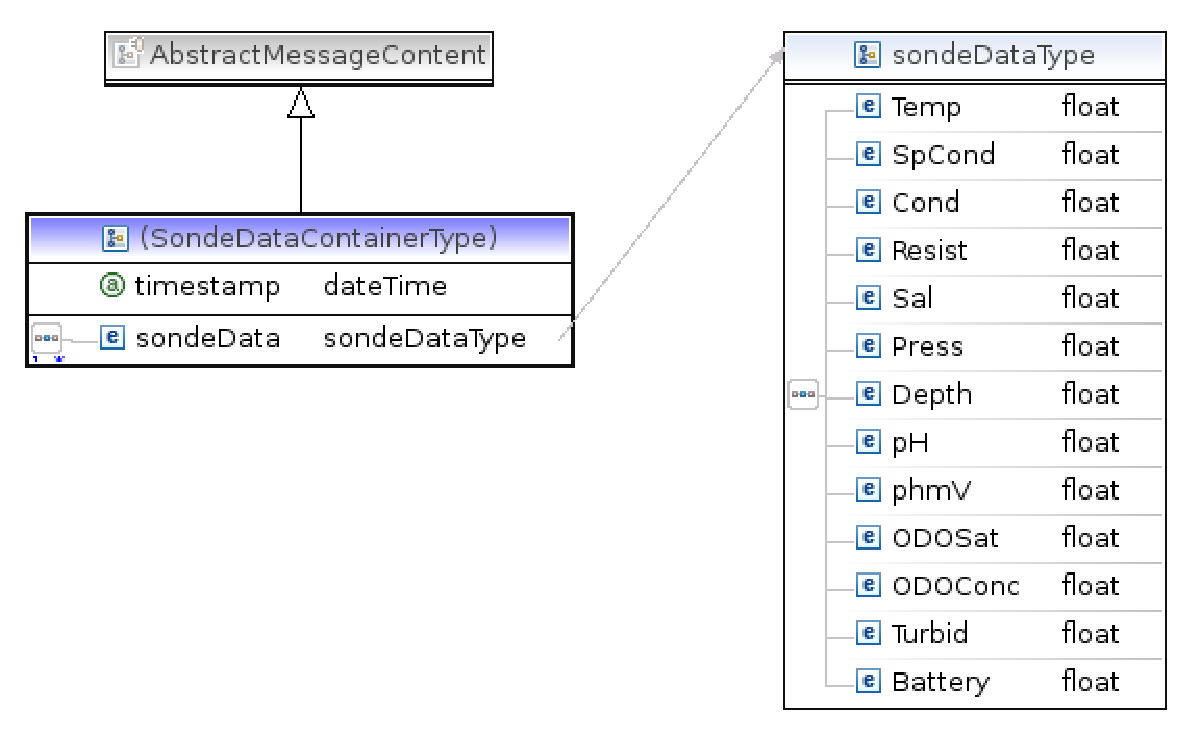
\epsfig{file=dsp-message-body-ysi, width=8cm, height=7cm}
\caption{\label{FIG_DSP_YSI_DATA} Structure of the YSI Component Data.}
\end{figure}

The schema describes two Java classes, sondeDataType and
SondeDataMessage, which are used to package the Sonde's incoming data
into a DSP message for delivery to a remote consumer.  The
SondeDataMessage class extends the AbstractMessageContent class by
adding a new type to the message payload, SondeDataType.  Each time
the Sonde transmits its payload of measurement data during a sampling
interval, the data is converted into a SondeDataType which is then
encapsulated within SondeDataMessage and then sent to a remote
consumer.

The YSI Sonde component can also be configured via special DSP
messages, to direct the Sonde to change its sampling frequency.  These
property messages originate from the web frontend that we will
explained in a subsequent section.

\subsection{Remote Communication}

After producing the SondeDataContainer data, the YSI Sonde component
will wrap it up in a DSP Message Message and pass it to the DSP Broker
for its delivery.  However, our use case scenario is that the message
must go from the local sensor device to the server. For this reason,
we have developed a pair of client and server DSP components
specialized in transferring and receiving serialized objects throught
the communication channel using the HTTP protocol \cite{RFC2068}.

\begin{itemize}
\item DSP Wire Transport Client: takes a collection of DSP messages
  and transmit them using an HTTP client API written in JAVA
  \cite{http-client}. As a non-functional requirement, a DSP
  administrator can set the interval in which this component will
  transmit messages to other components;
\item DSP Wire Transport Server: is implemented using the Java
  Servlets technology \cite{java-servlets}, and is used to receive the
  collection of DSP messages transmitted, and potentially send DSP
  messages back to the sensor station.
\end{itemize}

One of the non-functional requirements for the DSP is to maximize the
utilization of the communication channel. For this specific reason, we
opted to add the type Messages Container, which contains a collection
of DSP messages, and specific identifiers of the hosting sensor.
Figure \ref{FIG_DSP_MSGS_CONTAINER} contains the structure of the DSP
Messages Container.

\begin{figure}[!htb]
\centering
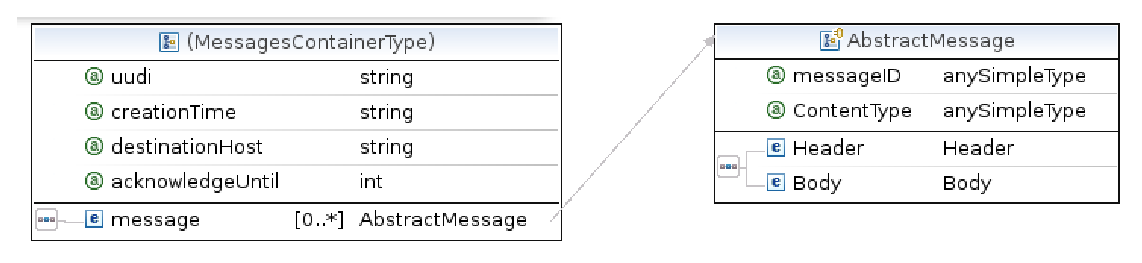
\epsfig{file=dsp-messages-container, width=8cm}
\caption{\label{FIG_DSP_MSGS_CONTAINER} The structure of Messages Container.}
\end{figure}

Some remarks regarding the Messages Container and it's implementation are as
follows:

\begin{itemize}
  \item Container with or without Messages Container: an instance of
  MessagesContainer may or may not have DSP messages;
  \item Container may be used to acknowledge messages using a similar strategy
  as the Slide Windowing protocol \cite{slide-window}. 
\end{itemize}

\subsection{Sending Messages Container}

It's important to note that, at this point, the DSP Broker had already
checked with the Matcher which are the DSP components that will be
receive a copy of the message in question. The matcher had specific
instructions to use the DSP Wire Transport Client component as the
default ``Proxy'' or default gateway, if you prefer.

By building a MessagesContainer instance, the Wire Transport Client
adds all the messages addressed to the ``destinationHost'', with
specific UUID of the component (2).

\subsection{Receiving Messages Container}

After the DSP Wire Transport Server receives the Messages Container
(3), it unmarshalls the messages and forward them to the local DSP
Broker.

The reception of those messages will ALWAYS depend on the local DSP Broker and
its combination with the Matcher. The steps (4), (5) and (6) are the
actual reception of DSP messages. Container might also include an attribute
called acknowledgeUntil, which determines the next actions that will occur in the system.

\subsection{Web Management}

Web Interface. Management messages are regular
DSPMessages. Asynchronous UI: UI may only build up after next
communication cycle.

\section{Conclusions and Outlook}
\label{SEC_CONCLUSION}

The California coastal region is populated by a vast number of
remotely deployed sensors that monitor environmental conditions
ranging from weather to water quality to ocean surface currents.
These sensors are operated by data providers, including resource
management groups, research scientists, municipalities, and state and
federal agencies, who could use near real-time data streams to inform
decision that impact public health, public safety, and the protection
of resources.  In addition, there are efforts underway at the state
and federal level to collate the data collected by the individual data
providers into integrated monitoring networks that will enhance the
distribution of monitoring data to public, private, and federal users
groups.  Success of these efforts, whether small scale or a large
integrated network, depends on the first step in the data management
process: reliably obtaining data in near real-time from remotely
located sensors.  This step can be the weak link in the data
management pathway when telemetry options are unreliable.  The
availability of a plug-and-play computing platform designed to
communicate with a variety of sensor types and to provide data
telemetry to distant brick and mortar data centers would stabilize
data streams with poor telemetry and allowing expansion of sensor
coverage into regions not presently served.  The low power consumption
and low cost of these units would be particularly beneficial for
applications with long service cycles and for data providers trying to
maintain data streams on a limited budget.

\bibliography{lit}
\bibliographystyle{plain}


\end{document}
